% !TEX root = ../probability_hse_exams.tex
\newpage
\thispagestyle{empty}
\section{Контрольная работа 1. ИП}


\subsection[2019-2020]{\hyperref[sec:sol_kr_01_ip_2019_2020]{2019-2020}}
\label{sec:kr_01_ip_2019_2020}


\begin{enumerate}
  \item Илон Маск подбрасывает правильную монетку до тех пор, пока не выпадет последовательность
  РОР. В процессе игры за каждого выброшенного «орла» Илон получает 100 тысяч долларов от компании Tesla.
  
  \begin{enumerate}
    \item Сколько в среднем денег зарабатывает Илон за одну игру?
    \item Как изменится ответ, если за каждого «орла», идущего подряд, выигрыш растёт на 100 тысяч,
    а промелькнувшая «решка» сбрасывает выигрыш за «орлов» до 100 тысяч?
  
  Пояснение: например, за ООРООО Илон получит $100 + 200 + 100 + 200 + 300$ тысяч долларов.
  \end{enumerate}
  
  
  \item Попугай Кеша подбрасывает кубик до первой шестёрки. 
  
  \begin{enumerate}
    \item Сколько в среднем подбрасываний ему потребуется?
    \item Сколько в среднем подбрасываний ему потребовалось, если известно, что
    пятерок в процессе игры выпало ровно две?
    \item Сколько в среднем подбрасываний ему потребовалось, если известно, что
    ни разу не выпадала нечётная грань?
  \end{enumerate}
  
  \item Илон Маск и Грета Тунберг оказались на Луне. 
  Судьба забросила их в случайные независимые точки, равномерно распределённые по поверхности Луны. 
  
  Илон Маск тут же бросился рыть совершенно прямой туннель к
  Грете. Диаметр Луны будем считать равным единице.
  
  Найдите функцию плотности длины туннеля $L$ для случаев:
  
  \begin{enumerate}
    \item Луна — плоская;
    \item Луна — объёмная.
  \end{enumerate}
  
  
  \item У Джеки Чана в коробке лежат бумажки с числами от 1 до 100. 
  Джеки Чан случайно извлекает 30 этих бумажек, без возвращения бумажек в коробку.
  Затем он считает среднее арифметическое извлечённых чисел, и получает случайную величину $Y$.
  
  Найдите $\E(Y)$, $\Var(Y)$.
  
  \item Преподаватель Николай Арефьеф любит короткие решения нетривиальных
  задач. 
  Однажды он пообещал студентам, что включит в контрольную
  работу задачу на новую тему с вероятностью $1/3$.
  
  У Николая есть только правильная монетка.
  
  \begin{enumerate}
  \item Какой эксперимент с монеткой позволяет выполнить данное обещание?
  \item Какова минимальная ожидаемая продолжительность подобного эксперимента?
  \end{enumerate}
  
  Перед контрольной Николай подбросил монетку два раза и на основании этих
  бросков принял решение о том, включить ли задачу в контрольную.
  
  \begin{enumerate}[resume]
    \item Попала ли задача в контрольную работу?
  \end{enumerate}
  
  
  \end{enumerate}
  



\subsection[2018-2019]{\hyperref[sec:sol_kr_01_ip_2018_2019]{2018-2019}}
\label{sec:kr_01_ip_2018_2019}

\begin{enumerate}
\item Пират Злопамятный Джо очень любит неразбавленный ром. Из-за того,
что он много пьёт, у него проблемы с памятью, и он помнит не больше,
чем три последних пинты. Хозяин таверны «Огненная зебра»
с вероятностью $1/8$ разбавляет каждую подаваемую пинту рома.
Если по ощущением Джо половина выпитых пинт или больше была разбавлена, то он
разносит таверну к чертям собачьим.
Только что Джо вошёл в таверну и закал первую пинту.

Сколько в среднем пинт выпьет Джо, прежде чем разнесёт таверну?

\item В таверне «Крутой ковбой» разбавленный ром подают с вероятностью $1/2$.
Джо немного сменил свой характер и теперь устраивает скандал,
если две пинты рома подряд разбавлены.

Какова вероятность того, что Джо сможет выпить 100 пинт подряд без скандалов?

\item Али-Баба хочет проникнуть в пещеру с сокровищами. Вход в
пещеру закрыт и его охраняет Джин с квадратным подносом.
В каждой вершине подноса — непрозрачный стаканчик. Под
каждым стаканчиком — монетка.
Если все четыре монетки окажутся в одинаковом положении, все —
орлом вверх, или все — решкой вверх, то вход откроется.
За одно действие Али-Баба может открыть любые два стаканчика и
положить открывшиеся монетки любой стороной вверх.
После действия Али-Бабы Джин накрывает монетки стаканчиками,
быстро-быстро вращает поднос и снова предоставляет поднос
Али-Бабе.
Углядеть за Джином или сделать пометки на подносе невозможно.

\begin{enumerate}
  \item Как надо действовать Али-Бабе, чтобы гарантировать себе вход в
  пещеру за наименьшее количество действий?
  \item Сколько действий
  потребуется в худшем случае?
\end{enumerate}

\item Злопамятный Джо очень любит играть в картишки. Перед Джо хорошо перемешанная
стандартная колода в 52 карты. Джо извлекает карты по одной.

На каком месте в среднем появляется первая Дама?

\item Вероятность того, что непросветлённый Ученик достигнет Просветления за малый интервал времени,
прямо пропорциональна длине этого интервала, а именно,
\[
\P(\text{достигнуть Просветления за отрезок времени }[t;t+\Delta]) =
0.2018 \Delta + o(\Delta)
\]

Какова точная вероятность того, что Ученик, начавший искать Просветление, так
и не достигнет его к моменту времени $t$?

\item Исследователь Василий выбирает равномерно и независимо друг от друга 10 точек на
отрезке $[0;1]$. Затем Василий записывает их координаты в порядке возрастания,
$Y_1 \leq Y_2 \leq \ldots \leq Y_{10}$.

Не производя вычислений, \textit{по определению},
выпишите функции плотности случайной величины $Y_4$.
\end{enumerate}


\newpage

\subsection[2017-2018]{\hyperref[sec:sol_kr_01_ip_2017_2018]{2017-2018}}
\label{sec:kr_01_ip_2017_2018}

Ровно 272 года назад императрица Елизавета повелела завезти во дворцы котов для ловли мышей.

\begin{enumerate}
\item В отсутствии кота Леопольда мыши Белый и Серый подкидывают по очереди
игральный додекаэдр.
%\footnote{Леопольд подсказывает по случаю праздника, что у додекаэдра 12 граней :)}
Сыр достаётся тому, кто первым выкинет число 6. Начинает подкидывать Белый.
\begin{enumerate}
  \item Какова вероятность того, что сыр достанется Белому?
  \item Сколько в среднем бросков продолжается игра?
  \item Какова дисперсия числа бросков?
\end{enumerate}

\item Микки Маус, Белый и Серый решили устроить труэль из любви к мышки Мии.
Сначала делает свой выстрел Микки, затем Белый, затем Серый, затем снова Микки и так до тех пор,
пока в живых не останется только один.

Прошлые данные говорят о том, что Микки попадает с вероятностью $1/3$,
Белый — с вероятностью $2/3$, а Серый стреляет без промаха.

Найдите оптимальную стратегию каждого мыша, куда кому следует целиться.

\item Микки Маус, Белый и Серый пойманый злобным котом Леопольдом до начала труэли.
И теперь Леопольд будет играть с ними в странную игру.

В комнате три закрытых внешне неотличимых коробки: с золотом, серебром и платиной.
Общаться после начала игры мыши не могут, но могут заранее договориться о стратегии.

Правила игры таковы. Кот Леопольд будет заводить мышей в комнату по очереди.
Каждый из мышей может открыть две коробки по своему выбору.
Перед следующим мышом коробки закрываются.

Если Микки откроет коробку с золотом, Белый — с серебром, а Серый — с платиной,
то они выигрывают. Если хотя бы один из мышей не найдёт свой металл, то Леопольд
их съест.
\begin{enumerate}
\item Какова оптимальная стратегия?
\item Какова вероятность выигрыша при использовании оптимальной стратегии?
\end{enumerate}

\item Накануне войны Жестокий Тиран Мышь очень большой страны издал указ.
Отныне за каждого новорождённого мыша-мальчика семья получает денежную премию,
но если в семье рождается вторая мышка-девочка, то всю семью убивают.
Бедные жители страны запуганы и остро нуждаются в деньгах, поэтому в каждой семье
мыши будут появляться до тех пор, пока не родится первая мышка-девочка.
\begin{enumerate}
  \item Каким будет среднее число детей в мышиной семье?
  \item Какой будет доля мышей-мальчиков в стране?
  \item Какой будет средняя доля мышей-мальчиков в случайной семье?
  \item Сколько в среднем мышей-мальчиков в случайно выбираемой семье?
\end{enumerate}

\item Вальяжный кот Василий положил на счёт в банке на Гаити один гурд.
Сумма на счету растёт непрерывно с постоянной ставкой в течение очень длительного
промежутка времени. В случайный момент этого промежутка кот Василий закрывает свой вклад.

Каков закон распределения первой цифры полученной Василием суммы?
\end{enumerate}



\newpage
\subsection[2016-2017]{\hyperref[sec:sol_kr_01_ip_2016_2017]{2016-2017}}
\label{sec:kr_01_ip_2016_2017}


\begin{enumerate}
\item Задача о макаронинах

В тарелке запутавшись лежат много-много макаронин.
Я по очереди связываю попарно все торчащие концы макаронин.
\begin{enumerate}
\item Какова примерно вероятность того, что я свяжу все макаронины в одно большое кольцо?
\item Сколько в среднем колец образуется?
\item Каково среднее число колец длиной в одну макаронину?
\end{enumerate}

\item Планета Плюк

На планету Плюк, окружность, в случайных точках садятся $n$ пепелацев.
Радиосвязь между двумя точками на планете Плюк возможна, если центральный угол
между этими двумя точками меньше $\pi/2$.
\begin{enumerate}
\item Какова вероятность того, что из любой точки планеты можно связаться хотя бы с одним пепелацем?
\item Какова вероятность того, что при $n=3$ все три пепелаца смогут поддерживать связь друг с другом (необязательно напрямую, возможно через посредника)?
\item Как изменятся ответы, если планета Плюк — это сфера?
\end{enumerate}

\item Чайник Рассела

Вокруг Солнца по эллиптической орбите вращается абсолютно плоский чайник Рассела
с площадью $42$ см$^2$. Летающий Макаронный Монстр проецирует чайник Рассела на
случайную плоскость.

Чему равна ожидаемая площадь проекции?

% \item Винни-Пух собирается играть в Пустяки и готовит для игры палочки. Он нашел
% палку длиной 1 м, а дальше поступает следующим образом. Разламывает палку равномерно
% в случайном месте, одну полученную часть использует для игры, а вторую снова случайным
% образом делит на две части. Далее одну новую часть Винни-Пух снова использует
% для игры, а вторую новую часть снова делит на две. И так далее. Обозначим $X_i$ —
% длину палочки, использованной Винни-Пухом в $i$-ых Пустяках.

% Найдите функцию плотности $X_i$, $\E(X_i)$, $\Var(X_i)$

\item Чак Норрис против Брюса Ли

Чак Норрис хватается за верёвку в форме окружности в произвольной точке.
Брюс Ли берёт мачете и с завязанными глазами разрубает верёвку в двух случайных
независимых местах. Чак Норрис забирает себе тот кусок, за который держится.
Брюс Ли забирает оставшийся кусок.  Вся верёвка имеет единичную длину.
\begin{enumerate}
\item Чему равна ожидаемая длина куска верёвки, доставшегося Брюсу Ли?
\item  Вероятность того, что у Брюса Ли верёвка длиннее?
\end{enumerate}

\item Истеричная певица

Начинающая певица дает концерты каждый день. Каждый её концерт приносит продюсеру
$0.75$ тысяч евро. После каждого концерта певица может впасть в депрессию
с вероятностью $0.5$. Самостоятельно выйти из депрессии певица не может.
В депрессии она не в состоянии проводить концерты. Помочь ей могут только хризантемы
от продюсера. Если подарить цветы на сумму $0\le x\le 1$ тысяч евро, то она выйдет
из депрессии с вероятностью $\sqrt{x}$.

Какова оптимальная стратегия продюсера, максимизирующего ожидаемую прибыль?

\item Гадалка

Джульетта пишет на бумажках два любых различных натуральных числа по своему выбору.
Одну бумажку она прячет в левую руку, а другую — в правую. Ромео выбирает любую руку
Джульетты. Джульетта показывает число, написанное на выбранной бумажке. Ромео высказывает
свою догадку о том, открыл ли он большее из двух чисел или меньшее. Ромео выигрывает,
если он угадал.

Приведите пример стратегии Ромео, дающей ему вероятность выигрыша строго больше
$0.5$ против любой стратегии Джульетты.

\item Мудрецы

В ряд друг за другом за бесконечным столом сидит счётное количество Мудрецов,
постигающих Истину. Первым сидит Абу Али Хусейн ибн Абдуллах ибн аль-Хасан ибн
Али ибн Сина:

\begin{figure}[h!]
  \begin{center}
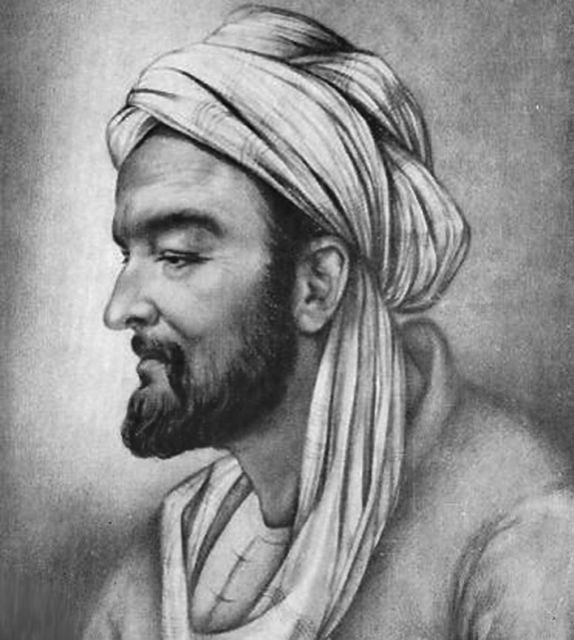
\includegraphics[width=5cm]{images/abu_ali.jpg}
  \caption*{«Коль смолоду избрал к заветной правде путь, \\
 С невеждами не спорь, советы их забудь». }
 \end{center}
\end{figure}

Каждый Мудрец может постигнуть Истину самостоятельно с вероятностью $1/9$
или же от соседа\footnote{Студенты постигают Истину примерно также!}. Независимо
от способа постижения Истины, просветлённый Мудрец поделится Истиной с соседом
слева с вероятностью $2/9$ и с соседом справа также с вероятностью $2/9$ (независимо
от соседа слева).
\begin{enumerate}
\item Какова вероятность того, что Абу Али Хусейн ибн Абдуллах ибн аль-Хасан ибн
Али ибн Сина постигнет Истину?
\item Как изменится ответ, если ряд Мудрецов бесконечен в обе стороны?
\end{enumerate}
\end{enumerate}



\newpage
\subsection[2015-2016]{\hyperref[sec:sol_kr_01_ip_2015_2016]{2015-2016}}
\label{sec:kr_01_ip_2015_2016}

\subsubsection*{Индивидуальный тур}

\begin{enumerate}
\item Для разминки вспомним греческий алфавит!

\begin{enumerate}
\item По-гречески — Σωκρατης, а по-русски — \underline{\hspace{2cm}}
\item Изобразите прописные и строчные буквы: эта \underline{\hspace{2cm}},
дзета \underline{\hspace{2cm}}, вега \underline{\hspace{2cm}},
шо \underline{\hspace{2cm}}. Если такой буквы в греческом нет, то поставьте прочерк.
\item Назовите буквы: τ \underline{\hspace{2cm}}, θ \underline{\hspace{2cm}},
ξ \underline{\hspace{2cm}}.
%\item Если пересчитать все буквы в греческом алфавите, то их окажется ровно \underline{\hspace{2cm}} %24
\end{enumerate}

\item Подбрасываются 2 симметричные монеты. Событие $A$ — на первой монете выпал герб,
событие $B$ — на второй монете выпал герб, событие $C$ — монеты выпали разными сторонами.
\begin{enumerate}
\item Будут ли эти события попарно независимы?
\item Сформулируйте определение независимости в совокупности для трех событий
\item Являются ли события $A$, $B$, $C$ независимыми в совокупности?
\end{enumerate}


\item Имеются два игральных кубика: \textbf{красный} со смещенным центром тяжести,
так что вероятность выпадения «6» равняется $1/3$, а оставшиеся грани имеют равные
шансы на появление и
правильный \textbf{белый} кубик.  Петя случайным образом выбирает кубик и подбрасывает его.
\begin{enumerate}
\item Вероятность того, что выпадет «6», равна \underline{\hspace{2cm}}
\item Вероятность того, что Петя взял красный кубик, если известно, что выпала шестерка,
равна \underline{\hspace{2cm}}
\item Если бы в эксперименте Петя подбрасывал  бы кубик не один раз, а 60 раз,
то безусловное математическое ожидание количества выпавших шестёрок равнялось бы
\underline{\hspace{2cm}}
\end{enumerate}

\begin{comment}
\item Неразменный пятак всегда выпадает «орлом». У Александра Привалова в кармане
один неразменный пятак и два обычных, равновероятно выпадающих «орлом» и «решкой».
Привалов достаёт одну из монет наугад не глядя.
\begin{enumerate}
\item Вероятность того, что он достанет неразменный пятак равна \underline{\hspace{2cm}} % 1/3
\item Не глядя на монету, Привалов подкидывает её. Вероятность того, что она выпадет
«орлом», равна \underline{\hspace{2cm}} % 2/3
%\item Если бы эту случайную монету подкинуть не один раз, а 10, то математическое ожидание числа «орлов» равнялось бы \underline{\hspace{2cm}} % 20/3
\item Наконец Привалов глядит на упавшую монету и видит, что выпал «орёл».
Вероятность того, что монета — неразменный пятак, равна \underline{\hspace{2cm}}
\end{enumerate}
\end{comment}

\item Винни-Пуху снится сон, будто он спустился в погреб, а там бесконечное
количество горшков. Каждый из них независимо от других может оказаться либо
пустым с вероятностью $0.8$, либо с мёдом с вероятностью $0.2$. Винни-Пух начинает
перебирать горшки по очереди в поисках полного. Хотя у него в голове и опилки,
Винни-Пух два раза в один и тот же горшок заглядывать не будет.
\begin{enumerate}
\item Вероятность того, что все горшки окажутся пустыми равна \underline{\hspace{2cm}}
\item Вероятность того, что полный горшок будет найден ровно с шестой попытки, равна \underline{\hspace{2cm}}
\item Вероятность того, что полный горшок будет найден на шестой попытке или ранее, равна \underline{\hspace{2cm}}
%\item Математическое ожидание числа перебранных горшков равняется \underline{\hspace{2cm}} % 5
\end{enumerate}

\item На самом деле у Винни-Пуха в погребе стоит 10 горшков. Каждый из них независимо
от других может оказаться либо пустым с вероятностью $0.8$, либо с мёдом с вероятностью
$0.2$.
\begin{enumerate}
\item Все десять горшков окажутся пустыми с вероятностью \underline{\hspace{2cm}}
\item Ровно $7$ горшков из десяти окажутся пустыми с вероятностью \underline{\hspace{2cm}}
\item Математическое ожидание числа горшков с мёдом равно \underline{\hspace{2cm}}
\end{enumerate}


\begin{comment}
\item Внутри треугольника с вершинами $(0,0)$, $(2,5)$ и $(8,0)$ случайно
равномерно по площади выбирается точка. Пусть $X$ и $Y$ — абсцисса и ордината
этой случаной точки.
\begin{enumerate}
\item Вероятность того, что $X>5$ равна \underline{\hspace{2cm}}.
\item Вероятность того, что $X>5$ и одновременно $Y<3$ равна \underline{\hspace{2cm}}.
\item Вероятность того, что $X>5$ если известно, что $Y<3$ равна \underline{\hspace{2cm}}.
\item События $X>5$ и $Y<3$ являются \underline{\hspace{1cm}}висимыми.
\item Функция плотности величины $X$ равна \underline{\hspace{2cm}}
\end{enumerate}
\end{comment}

\item В галактике Флатландии все объекты двумерные. На планету Тау-Слона (окружность)
в случайных точках независимо друг от друга садятся три корабля. Любые два корабля
могут поддерживать прямую связь между собой, если центральный угол между ними меньше
прямого.
\begin{enumerate}
\item Вероятность того, что первый и второй корабли могут поддерживать прямую
связь равна \underline{\hspace{2cm}}
\item Вероятность того, что все корабли смогут поддерживать прямую связь друг
с другом равна \underline{\hspace{2cm}}
\item Вероятность того, что все корабли смогут поддерживать прямую связь друг
с другом, если первый и второй корабль могут поддерживать прямую связь, равна
\underline{\hspace{2cm}}
\end{enumerate}
Подсказка: во Флатландии хватит рисунка на плоскости, ведь координату третьего
корабля можно принять за\ldots

\item Время (в часах), за которое студенты выполняют экзаменационное задание
является случайной величиной $X$ с функцией плотности
\[
f(x)=\begin{cases}
3x^2, \, \text{ если } x \in [0;1] \\
0, \, \text{ иначе }
\end{cases}
\]

\begin{enumerate}
\item Функция распределения случайной величины $X$ равна \underline{\hspace{2cm}}
\item Вероятность того, что случайно выбранный студент закончит работу менее чем
за полчаса равна \underline{\hspace{2cm}}.
\item Медиана распределения равна \underline{\hspace{2cm}}
\item Вероятность того, что студент, которому требуется по меньшей мере 15 минут
для выполнения задания, справится с ним более, чем за 30 минут, равна \underline{\hspace{2cm}}
\item Функция распределения случайной величины $Y=1/X$ равна \underline{\hspace{2cm}}
\item Функция плотности случайной величины $Y=1/X$ равна \underline{\hspace{2cm}}
\end{enumerate}
\end{enumerate}

\subsubsection*{Командный тур}

\begin{enumerate}
\item Восьминогий Кракен. У Кракена 8 ног-шупалец. Если отрубить одно щупальце,
то в замен него с вероятностью $1/4$ вырастает новое; с вероятностью $1/4$ вырастает
два новых; с вероятностью $1/2$, слава Океану, не вырастает ничего.

Против Кракена бьётся сам Капитан! Он наносит точные удары и безупречно умело
уворачивается от ударов Кракена.
\begin{enumerate}
\item Какова вероятность того, что Капитан победит, отрубив ровно 10 щупалец?
\item Какова вероятность того, что бой Кракена и Капитана продлится вечно?
\item Сколько щупалец в среднем отрубит Капитан прежде чем победит?
\end{enumerate}

\item Разбавленный ром. Пират Злопамятный Джо очень любит неразбавленный ром. Из-за
того, что он много пьёт, у него проблемы с памятью, и он помнит не
больше, чем три последних пинты. Хозяин таверны с вероятностью $1/4$ разбавляет
каждую подаваемую пинту рома. Если по ощущением Джо половина выпитых
пинт или больше была разбавлена, то он разносит таверну к чертям собачьим.
\begin{enumerate}
\item Какова вероятность того, что хозяин таверны не успеет подать Джо третью пинту рома?
\item Сколько в среднем пинт выпьет Джо, прежде чем разнесёт таверну?
\end{enumerate}

\item $XY$ в степени $Z$. Чтобы поступить на службу Её Величества, пиратам предлагается
следующая задача. Случайные величины $X$, $Y$ и $Z$ равномерны на отрезке $[0;1]$
и независимы.
\begin{enumerate}
\item Найдите функцию распределения случайной величины $-\ln X$
\item Найдите функцию распределения случайной величины $-(\ln X + \ln Y)$
\item Найдите функцию распределения случайной величины $-Z(\ln X + \ln Y)$
\item Какое распределение имеет случайная величина $(XY)^Z$?
\end{enumerate}

\item Тортики. Пираты очень любят тортики и праздновать день рождения! Если хотя
бы у одного пирата на корабле день рождения, то все, включая капитана, празднуют
и кушают тортики. Корабль в праздничный день дрейфует под действием ветра и не факт,
что в нужном направлении.
\begin{enumerate}
\item Сколько пиратов нужно нанять капитану, чтобы ожидаемое количество праздничных
дней было равно 100?
\item Сколько пиратов нужно нанять капитану, чтобы максимизировать ожидаемое количество
рабочих пирато-дней (произведение числа пиратов на число рабочих дней)?
\end{enumerate}

\item Девятый вал. На побережье пиратского острова одна за одной набегают волны.
Высота каждой волны — равномерная на $[0;1]$ случайная величина. Высоты волн независимы.
Пираты называют волну «большой», если она больше предыдущей и больше следующей.
Пираты называют волну «рекордной», если она больше всех предыдущих волн от начала
наблюдения. Обозначим события $B_i= \{ i\text{-ая волна была большой} \}$ и
$R_i=\{ i\text{-ая волна была рекордной} \}$.
\begin{enumerate}
\item Найдите $\P(R_{100})$, $\P(B_{100})$
\item Капитан насчитал 100 волн. Сколько в среднем из них были «рекордными»?
\item Найдите $\P(R_{99} | R_{100})$, $\P(R_{100}|B_{100})$
\end{enumerate}

\item Три сундука. Три пирата, Генри Рубинов, Френсис Пиастров и Эдвард Золотов
играют одной командой в игру. В комнате в ряд, слева направо, стоят в случайном
порядке три закрытых внешне неотличимых сундука: с рубинами, пиастрами и золотом.
Общаться после начала игры они не могут, но могут заранее договориться о стратегии.
Они заходят в комнату по очереди. Каждый из них может открыть два сундука по своему
выбору. После каждого пирата комната возвращается уборщицей идеально точно в исходное
состояние. Если Рубинов откроет коробку с рубинами, Писатров — с пиастрами, а Золотов —
с золотом, то их команда выигрывает. Если хотя бы один из пиратов не найдёт свою цель,
то их команда проигрывает.
\begin{enumerate}
\item Какова вероятность выигрыша, если все пираты пробуют открыть первый и второй сундуки?
\item Какова оптимальная стратегия?
\item Какова вероятность выигрыша при использовании оптимальной стратегии?
\end{enumerate}
\end{enumerate}


\newpage
\subsection[2014-2015]{\hyperref[sec:sol_kr_01_ip_2014_2015]{2014-2015}}
\label{sec:kr_01_ip_2014_2015}

\subsubsection*{ Часть 1}

\begin{enumerate}
%\item Винни-Пух собирается играть в Пустяки и готовит для игры палочки. Он нашел палку длиной 1 м, а дальше поступает следующим образом. Разламывает палку равномерно в случайном месте, одну полученную часть использует для игры, а вторую снова случайным образом делит на две части. Далее одну новую часть Винни-Пух снова использует для игры, а вторую новую часть снова делит на две. И так далее. Обозначим $X_i$ — длину палочки, использованной Винни-Пухом в $i$-ых Пустяках.

%Найдите функцию плотности $X_i$, $\E(X_i)$, $\Var(X_i)$

\item Вася купил два арбуза у торговки тёти Маши и один арбуз у торговки тёти Оли.
Арбузы у тёти Маши спелые с вероятностью 90\% (независимо друг от друга), арбузы
у тёти Оли спелые с вероятностью 70\%.
\begin{enumerate}
\item Какова вероятность того, что все Васины арбузы спелые?
\item Придя домой Вася выбрал случайным образом один из трех арбузов и разрезал его.
Какова вероятность того, что это арбуз от тёти Маши, если он оказался спелым?
\item Какова вероятность того, что второй и третий съеденные Васей арбузы были от
тёти Маши, если все три арбуза оказались спелыми?
\end{enumerate}


\item В большой большой стране живет очень большое количество $n$ семей.
Количества детей в разных семьях независимы. Количество детей в каждой семье —
случайная величина с распределением заданным табличкой:

\begin{center}
\begin{tabular}{ccccc}
\toprule
$x$ & $0$ & $1$ & $2$ & $3$ \\ \midrule
$\P(X=x)$ & $0.1$ & $0.3$ & $0.2$ & $0.4$ \\ \bottomrule
\end{tabular}
\end{center}

\begin{enumerate}
\item Исследователь Афанасий выбирает одну семью из всех семей наугад, пусть $X$ —
число детей в этой семье. Найдите $\E(X)$ и $\Var(X)$.
\item Исследователь Бенедикт выбирает одного ребенка из всех детей наугад, пусть $Y$ —
число детей в семье этого ребёнка. Как распределена величина $Y$? Что больше,
$\E(Y)$ или $\E(X)$?
\end{enumerate}

\item Функция плотности случайной величины $X$ имеет вид
\[
f(x)=
\begin{cases}
\frac{3}{8} x^2, \text{ если } x\in [0;2] \\
0, \text{ иначе }
\end{cases}
\]
\begin{enumerate}
\item Не производя вычислений найдите $\int_{-\infty}^{+\infty}f(x)\,dx$
\item Найдите $\E(X)$, $\E(X^2)$ и дисперсию $\Var(X)$
\item Найдите $\P(X>1.5)$, $\P(X>1.5 \mid X>1)$
\item При каком $c$ функция $g(x)=c x f(x)$ будет функцией плотности некоторой
случайной величины?
\end{enumerate}

\item Известно, что  $\E\left(Z\right)=-3$, $\E\left(Z^{2} \right)=15$,
$\Var\left(X+Y\right)=20$  и  $\Var\left(X-Y\right)=10$.
\begin{enumerate}
\item Найдите $\Var\left(Z\right)$, $\Var\left(4-3Z\right)$ и
$\E\left(5+3Z-Z^{2} \right)$.
\item Найдите $\Cov\left(X,Y\right)$ и $\Cov\left(6-X,3Y\right)$.
\item Можно ли утверждать, что случайные величины $X$ и $Y$ независимы?
\end{enumerate}

\item Листая сборник задач по теории вероятностей Вася наткнулся на задачу:

\fbox{%
\parbox{15cm}{%
Какова вероятность того, что наугад выбранный ответ на этот вопрос окажется верным?

1) $0.25$		2) $0.5$		3) $0.6$		4) $0.25$ }
}

Чему же равна вероятность выбора верного ответа?

\item Книга в 500 страниц содержит 400 опечаток. Предположим, что каждая из них
независимо от остальных опечаток может с одинаковой вероятностью оказаться на любой
странице книги.
\begin{enumerate}
\item Определите вероятность того, что на 13-й странице будет не менее двух опечаток,
в явном виде и с помощью приближения Пуассона.
\item Определите наиболее вероятное число, математическое ожидание и дисперсию
числа опечаток на 13-ой странице.
\item Является ли 13-ая страница более «несчастливой», чем все остальные (в том
смысле, что на 13-ой странице ожидается большее количество очепяток, чем на любой другой)?
\end{enumerate}

\item Вася случайным образом посещает лекции по ОВП (Очень Важному Предмету).
С вероятностью $0.9$ произвольно выбранная лекция полезна, и с вероятностью $0.7$
она интересна. Полезность и интересность — независимые друг от друга и от номера
лекции свойства. Всего Вася прослушал 30 лекций.
\begin{enumerate}
\item Определите математическое ожидание и дисперсию числа полезных лекций,
прослушанных Васей
\item Определите математическое ожидание числа одновременно бесполезных и
неинтересных лекций, прослушанных Васей, и математическое ожидание числа лекций,
обладающих хотя бы одним из свойств (полезность, интересность).
\end{enumerate}
\item Функция распределения случайной величины X задана следующей формулой:
 \[
 F(x)=\frac{ae^x}{1+e^x}+b
 \]
Определите: константы $a$ и $b$, математическое ожидание и третий начальный
момент случайной величины $X$, медиану и моду распределения.

%\item Вы хотите приобрести некую фирму. Стоимость фирмы для ее нынешних владельцев — случайная величина, равномерно распределенная на отрезке $[0;1]$. Вы предлагаете владельцам продать ее за называемую Вами сумму. Владельцы либо соглашаются, либо нет. Если владельцы согласны, то Вы платите обещанную сумму и получаете фирму. Когда фирма переходит в Ваши руки, ее стоимость сразу возрастает на 20\%.

%\begin{enumerate}
%\item Чему равен Ваш ожидаемый выигрыш, если Вы предлагаете цену 0.5?
%\item Какова оптимальная предлагаемая цена?
%\end{enumerate}
\end{enumerate}

\subsubsection*{Часть 2}

\begin{enumerate}
\item Маша подкидывает кубик до тех пор, пока два последних броска в сумме не
дадут\footnote{Изначально вместо 12 задумывалось число 10, но  опечатка была
замечена поздно, поэтому решение приводится для 12.} 12. Обозначим случайные
величины: $N$ — количество бросков, а $S$ — сумма набранных за всю игру очков.
\begin{enumerate}
\item Найдите $\P(N=2)$, $\P(N=3)$
\item Найдите $\E(N)$, $\E(S)$, $\E(N^2)$
\item Пусть $X_N$ — результат последнего броска. Как распределена случайная
величина $X_N$?
\end{enumerate}


\item В столовую пришли 30 студентов и встали в очередь в случайном порядке.
Среди них есть Вовочка и Машенька. Пусть $V$ — это количество человек в очереди
перед Вовочкой, а $M\geq 0$ — количество человек между Вовочкой и Машенькой.
\begin{enumerate}
\item Найдите $\P(V=1)$, $\P(M=1)$, $\P(M=V)$
\item Найдите $\E(V)$, $\E(M)$, $\Var(M)$
\end{enumerate}

\item Польский математик Стефан Банах имел привычку носить в каждом из двух
карманов пальто по коробку спичек. Всякий раз, когда ему хотелось закурить трубку,
он выбирал наугад один из коробков и доставал из него спичку. Первоначально в каждом
коробке было по $n$ спичек. Но когда-то наступает момент, когда выбранный наугад
коробок оказывается пустым.
\begin{enumerate}
\item Какова вероятность того, что в другом коробке в этот момент осталось ровно
$k$ спичек?
\item Каково среднее количество спичек в другом коробке?
\end{enumerate}

\item Производитель чудо-юдо-йогуртов наклеивает на каждую упаковку одну из 50
случайно выбираемых наклеек. Покупатель собравший все виды наклеек получает приз
от производителя. Пусть $X$ — это количество упаковок йогурта, которое нужно купить,
чтобы собрать все наклейки.

Найдите $\P(X=50)$, $\E(X)$, $\Var(X)$

Hint: $\ln(50)\approx 3.91$, а $\sum_{i=1}^n \frac{1}{i} \approx \int_1^n \frac{1}{x}\, dx$ :)

\item В самолете $n$ мест и все билеты проданы. Первой в очереди на посадку стоит
Сумасшедшая Старушка. Сумасшедшая Старушка несмотря на билет садиться на случайно
выбираемое место. Каждый оставшийся пассажир садится на своё место, если оно свободно
и на случайное выбираемое место, если его место уже кем-то занято.
\begin{enumerate}
\item Какова вероятность того, что все пассажиры сядут на свои места?
%\item Какова вероятность того, что второй пассажир в очереди сядет на своё место?
\item Какова вероятность того, что последний пассажир сядет на своё место?
\item Чему примерно равно среднее количество пассажиров севших на свои места?
\end{enumerate}
\end{enumerate}



\newpage
\subsection[2013-2014]{\hyperref[sec:sol_kr_01_ip_2013_2014]{2013-2014}}
\label{sec:kr_01_ip_2013_2014}

\subsubsection*{Часть 1}

\begin{enumerate}

\item В жюри три человека, они должны одобрить или не одобрить конкурсанта.
Два члена жюри независимо друг от друга одобряют конкурсанта с одинаковой
вероятностью $p$. Третий член жюри  для вынесения решения бросает правильную монету.
Окончательное решение выносится большинством голосов.
\begin{enumerate}
\item С какой вероятностью жюри одобрит конкурсанта?
\item Что выгоднее для  конкурсанта: чтобы решение принимало данное жюри, или
чтобы решение принимал один человек, одобряющий с вероятностью $p$?
\end{enumerate}

\item Вероятность застать Васю на лекции зависит от того, пришли ли на лекцию
Маша и Алена. Данная вероятность равна $p$, если девушек нет; $5p$ — если обе
девушки пришли на лекцию; $3p$ — если пришла только Маша и $2p$ — если пришла
только Алена. Маша и Алена посещают лекции независимо друг от друга с вероятностями
$0.6$ и $0.3$ соответственно.
\begin{enumerate}
\item Определите вероятность того, что на лекции присутствует Алёна,
если в аудитории есть Вася.
\item Кого чаще можно застать на тех лекциях, на которых присутствует Вася:
Машу или Алёну?
\item При каком значении $p$ Вася посещает половину всех лекций?
\end{enumerate}

\item Страховая компания страхует туристов, выезжающих за границу, от невыезда
и наступления страхового медицинского случая за границей. Застраховано 100 туристов.
Вероятность «невыезда» за границу случайно выбранного туриста — $0.002$,
а страховые выплаты в этом случае — 2000 у.е.; вероятность обращения за медицинской
помощью за границей — $0.01$, а страховые выплаты — 3000 у.е.
\begin{enumerate}
\item Определите вероятность того, что ровно пятеро туристов не смогут выехать за границу.
\item Найдите математическое ожидание, дисперсию и наиболее вероятное число не выехавших туристов.
\item Вычислите математическое ожидание и дисперсию величины совокупных страховых выплат
\item Вычислите ковариацию между выплатами по двум видам страхования.
\end{enumerate}

\item Известно, что  $\E(X)=-1$, $\E(Y)=1$, $\Var(X)=9$, $\Var(Y)=4$, $\Corr(X,Y)=1$.
Найдите
\begin{enumerate}
\item $\E(Y-2X-3)$, $\Var(Y-2X-3)$
\item  $\Corr(Y-2X-3,X)$
\item Можно ли выразить $Y$ через $X$? Если да, то запишите уравнение связи.
\end{enumerate}

\item Совместное распределение доходов акций двух компаний $Y$ и $X$ задано в виде
таблицы
\begin{center}
\begin{tabular}{@{}cccc@{}}
\toprule
    & $X=-1$ & $X=0$ & $X=1$ \\ \midrule
$Y=-1$ & $0.1$  & $0.2$   & $0.2$ \\
$Y=1$ & $0.2$  & $0.1$ & $0.2$ \\ \bottomrule
\end{tabular}
\end{center}

Найдите:
\begin{enumerate}
\item Частные распределения случайных величин $X$ и $Y$
\item $\Cov(X,Y)$
\item Можно ли утверждать, что случайные величины $X$ и $Y$ зависимы?
\item У инвестора портфель, в котором доля акций $X$ составляет $\alpha$,
а доля акций $Y$ — $(1-\alpha)$. Каковы должны быть доли, чтобы риск портфеля
(дисперсия дохода) был бы минимальным?
\item Условное распределение случайной величины $X$ при условии $Y=-1$.
\item Условное математическое ожидание $\E(X\mid Y=-1)$
\end{enumerate}
\item Докажите, что из сходимости в среднем порядка $s>0$ следует сходимость
по вероятности.
\end{enumerate}


\subsubsection*{Часть 2}

\begin{enumerate}
\item Муравей находится внутри спичечного коробка, в вершине $A$. В противоположной
вершине $B$ есть маленькая дырочка, через которую муравей сможет выбраться на поверхность.
В вершине $C$, соседней с вершиной $A$, лежит крупинка сахара. Муравей ползает
только по рёбрам коробка, выбирая каждый раз равновероятно одно из доступных в
вершине рёбер наугад. Например, он может поползти обратно.
\begin{enumerate}
\item Какова вероятность того, что муравей найдет крупинку сахара до того, как выберется?
\item Сколько в среднем перемещений понадобится муравью, чтобы выбраться?
\item Какова дисперсия количества перемещений, которые понадобятся муравью, чтобы
выбраться?
\end{enumerate}

\item В очереди стояло $20$ человек, когда касса внезапно закрылась. Поэтому $10$
случайных людей из очереди решили покинуть очередь. В результате этого очередь
оказалась разбита на случайное число кусков $X$. Найдите $\E(X)$, $\Var(X)$.

\item Предположим, что три возможных генотипа \verb|aa|, \verb|Aa| и \verb|AA|
изначально встречаются с частотами $p_1$, $p_2$ и $p_3$, где $p_1 + p_2 + p_3 = 1$.
Ген не сцеплен с полом, поэтому частоты $p_1$, $p_2$ и $p_3$ одинаковы для мужчин
и для женщин.
\begin{enumerate}
\item У семейных пар из этой популяции рождаются дети. Назовём этих детей первым
поколением. Каковы частоты для трёх возможных генотипов в первом поколении?
\item У семейных пар первого поколения тоже рождаются дети. Назовём этих детей
вторым поколением. Каковы частоты для трёх возможных генотипов во втором поколении?
\item Каковы частоты для трёх возможных генотипов в $n$-ном поколении?
\item Заметив явную особенность предыдущего ответа сформулируйте теорему о равновесии
Харди-Вайнберга. Прокомментируйте утверждение: «Любой рецессивный ген со временем
исчезнет».
\end{enumerate}

\item Световая волна может быть разложена на две поляризованные составляющие,
вертикальную и горизонтальную. Поэтому состояние отдельного поляризованного фотона
может быть описано\footnote{На самом деле внутренний мир фотона гораздо разнообразнее.}
углом $\alpha$. Поляризационный фильтр описывается углом поворота $\theta$. Фотон
в состоянии $\alpha$ задерживается поляризационным фильтром с параметром $\theta$
с вероятностью $p=\sin^2(\alpha-\theta)$ или проходит сквозь фильтр с вероятностью
$1 - p$, переходя при этом в состояние $\theta$.

\begin{enumerate}
\item Какова вероятность того, что поляризованный фотон в состоянии $\alpha$ пройдёт
сквозь фильтр с параметром $\theta=0$?
\item Имеется два фильтра и поляризованный фотон в состоянии $\alpha$. Первый
фильтр — с $\theta=0$, второй — c $\theta=\pi/2$. Какова вероятность того, что
фотон пройдет через оба фильтра?
\item Имеется три фильтра и поляризованный фотон в состоянии $\alpha$. Первый
фильтр — с $\theta=0$, второй — c $\theta=\beta$, третий — с $\theta=\pi/2$.
Какова вероятность того, что фотон пройдет через все три фильтра? При каких $\alpha$
и $\beta$ она будет максимальной и чему при этом она будет равна?
\item Объясните следующий фокус. Фокусник берет два специальных стекла и видно,
что свет сквозь них не проходит. Фокусник ставит между двумя стёклами третье, и
свет начинает проходить через три стекла.
\end{enumerate}
\end{enumerate}
